\documentclass[12pt]{beamer}

\usepackage[T1]{fontenc}
\usepackage[utf8]{inputenc}
\usepackage[english,ngerman]{babel}
\usepackage{mathtools}
\usepackage{amsthm}
\usepackage{libertine}
\usepackage[libertine]{newtxmath}
\usepackage[mathscr]{euscript}
\usepackage{tikz-cd}
\usetikzlibrary{decorations.markings}
\usepackage{float}
\usepackage{listings}
\usepackage{xcolor}

\usepackage[scaled=0.9]{inconsolata}



%% ------------- Bibliography -------------
\usepackage[
backend=biber,
style=alphabetic,
maxnames=10,
maxalphanames=10]{biblatex}
\addbibresource{../bibliography.bib}
\usepackage{hyperref}
\urlstyle{same}


%% ------------- Beamer style settings -------------
%\usefonttheme{serif}
\usetheme{Singapore}
\usecolortheme{rose}

%Deactivating navigation symbols
\setbeamertemplate{navigation symbols}{}


% Deactivate the shading at the top of slide
% \newcommand{\removeheadshading}[0]{%
% 	\setbeamertemplate{headline}{%
% 		\begin{beamercolorbox}{section in head/foot}%
% 			\vskip2pt\insertnavigation{\paperwidth}\vskip2pt%
% 		\end{beamercolorbox}%
% 	}%
% }
% \removeheadshading
\setbeamertemplate{headline}{}


%% ------------- Math commands -------------
% New math commands
\DeclareMathOperator{\img}{Im}
\DeclareMathOperator{\sign}{sign}
\DeclareMathOperator{\id}{Id}
\DeclareMathOperator{\vol}{vol}
\DeclareMathOperator{\hodgestar}{\ast}
\DeclareMathOperator{\Hom}{Hom}

\newcommand{\interior}[1]{{\kern0pt#1}^{\mathrm{o}}}
\newcommand{\into}{\hookrightarrow}
\newcommand{\onto}{\twoheadrightarrow}
\newcommand{\opartial}{{\overline{\partial}}}

%% ---------------- Code design --------------------
\definecolor{codebg}{RGB}{245,245,245}
\definecolor{codeblue}{RGB}{36,36,140}
\definecolor{codegreen}{RGB}{0,120,0}

\lstset{
    backgroundcolor=\color{codebg},
    basicstyle=\ttfamily\small,
    keywordstyle=\color{codeblue}\bfseries,
    commentstyle=\color{codegreen},
    stringstyle=\color{red},
    frame=single,
    rulecolor=\color{black!20},
    breaklines=true,
    showstringspaces=false,
    tabsize=4
}

%% ------------- Settings fpr document -------------
\title[Classification of Handwritten Digits Stochastic Gradient Descent]{Classification of Handwritten Digits using Stochastic Gradient Descent}
\author{Álvaro Galisteo Bermúdez, Daniel Rath}
%\institute{Albert-Ludwigs-Universit\"{a}t Freiburg}
\date{16.02.2026}

\makeatletter
\hypersetup{
	pdftitle={@title},
	colorlinks,
	linkcolor=[rgb]{0.2,0.2,0.6},
	citecolor=[rgb]{0.2,0.6,0.2},
	urlcolor=[rgb]{0.6,0.2,0.2}}
\makeatother

\begin{document}

	% Title Page
	\frame{\titlepage}
	
	% Table of contents Maybe delete this one
%	\begin{frame}
%		\frametitle{Überblick}
%		\tableofcontents
%	\end{frame}

    \begin{frame}[fragile]
        \frametitle{The Dataset}
        The dataset contains $1797$ grayscale $8\times 8$ images of handwritten digits. Each associated with a label. 
        \begin{figure}
            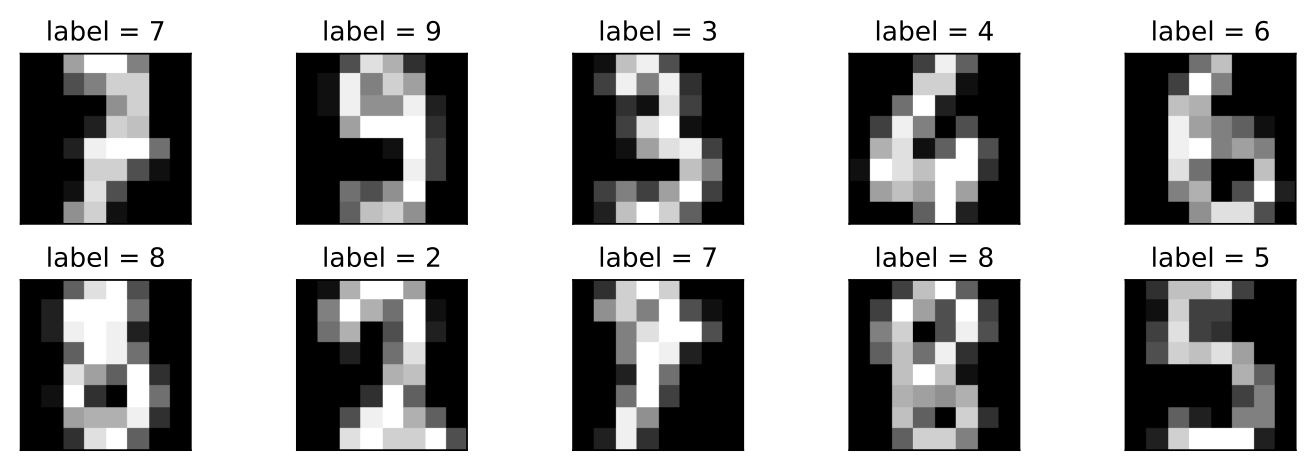
\includegraphics[scale=0.46]{dataset.png}
        \end{figure}
        It is available in python through the sklearn library
        \begin{lstlisting}[language=Python]
from sklearn.datasets import load_digits
        \end{lstlisting}
    \end{frame}

    \begin{frame}
        \frametitle{Multiclass Logistic regression - I}
        We represent the label $y_j$ of the image $a_j$ as 
        \begin{align*}
            p_j \in \mathbb{R}^{10}, \quad (p_j)_i = \begin{cases}
                1 & \text{if } i = y_j \\
                0 & \text{otherwise}
            \end{cases}
        \end{align*}
        The scores are given as
        \begin{align*}
            \varphi(a_j,x)_i = a_j^T w_i + b_i \qquad  \text{with  } x=(w_i,b_i)_{i=1}^{10}  w_i \in \mathbb{R}^{64}, b_i \in \mathbb{R}
        \end{align*}
        The prediction is given by
        \begin{align*}
            \tilde{y}_j = \underset{i\in\{0,\ldots,9\}}{\arg\max}\; \varphi(a_j;x)_i
        \end{align*}
        We interpret the scores as probabilities by
        \begin{align*}            
            \sigma(\varphi(a_j;x))_i = \frac{\exp(\varphi(a_j;x)_i)}{\sum_{l=0}^{9} \exp(\varphi(a_j;x)_l)}        
        \end{align*}
    \end{frame}

     \begin{frame}
        \frametitle{Multiclass Logistic regression - II}
        \begin{block}{The Optimization problem}
        The optimization problem we want to solve is
        \begin{align*} 
            \underset{x\in(\mathbb{R}^{64}\times \mathbb{R})^{10}}{\text{minimize }} \frac{1}{N}\sum_{j=1}^N L(p_j,\varphi(a_j;x)),
        \end{align*}
        where $L$ is the cross-entropy loss defined as
        \begin{align*}
            L(p,s) = \log\!\Big(\sum_{l=0}^{9} \exp\big(s_l\big)\Big) - \sum_{i=0}^{9} p_i s_i
        \end{align*}
        \end{block}
    \end{frame}

    \begin{frame}
        \frametitle{Cross entropy loss}
        \begin{beamercolorbox}[rounded=false,shadow=false]{block body}
        \begin{align*}
            \vspace{-5cm}
            L(p,s) = \log\!\Big(\sum_{l=0}^{9} \exp\big(s_l\big)\Big) - \sum_{i=0}^{9} p_i s_i
        \end{align*}
        \end{beamercolorbox}
        Using the cross-entropy loss ensures some important properties:
        \begin{itemize}
            \item Convexity of the optimization problem
            \item Differentiability for gradient descent methods
            \item Maximization of the likelihood of the observed data during training
        \end{itemize}

        Also note that we do not use the $\tilde{y} = \arg\max_{i \in \{0,\ldots,9\}}\; \varphi(a_j;x)_i$ in the loss function, because it is not differentiable.    
    \end{frame}
    \begin{frame}
        \frametitle{$L^2$-Regularization}
        To prevent overfitting we add an $L^2$-regularization term to the optimization problem:
        \begin{block}{The Regularized Optimization problem}
        \vspace{-0.5cm}
        \begin{align*}
            \underset{x\in(\mathbb{R}^{64}\times \mathbb{R})^{10}}{\text{minimize }} \frac{1}{N}\sum_{j=1}^N L(p_j,\varphi(a_j;x)) + \frac{\lambda}{2} \sum_{i=0}^{9} \|w_i\|^2
        \end{align*}
        \end{block}
         where $\lambda > 0$ is the regularization parameter.
        The regularization leads to
        \begin{itemize}
            \item smaller weights, which can help in generalization and prevent overfitting
            \item a unique finite optimum even if the data is linearly separable
            \item (numerically more stable optimization problem)
        \end{itemize}
    \end{frame}

    \begin{frame}
        \frametitle{Stochastic Gradient Descent}
        For solving the optimization problem we use Stochastic Gradient Descent (SGD), i.e. we choose a mini-batch $\mathcal{B}_k$ of size $B$ and calculate a stochastic estimator of the gradient as
        \begin{align*}
            \nabla L(x) = \frac{1}{B} \sum_{j \in \mathcal{B}_k} \nabla L(p_j, \varphi(a_j;x))
        \end{align*}
        The update is then given by
        \begin{align*}
            x^{k+1} = x^k - \eta_k \nabla L(x^k)
        \end{align*}
        This approach has some advantages and disadvantages, e.g.:
        \begin{itemize}
            \item Computationally efficient for larger datasets and small $B$
            \item Gradient can be to noisy if $B$ is too small
        \end{itemize}
    \end{frame}
    \begin{frame}[fragile]
    \frametitle{SGD Implementation (Mini-batch) --- I}
    \small
    \textbf{Finite-sum objective (training set).}\;
    \[
    f_\lambda(W,b)
    =
    \frac{1}{N}\sum_{j=1}^{N} L\!\big(y_j,\; a_j^\top W + b\big)
    +\frac{\lambda}{2}\,\|W\|_F^2,
    \qquad
    W\in\mathbb{R}^{64\times 10},\; b\in\mathbb{R}^{10}.
    \]

    \vspace{0.15cm}
    \textbf{Mini-batch gradient and update.}\;
    For a mini-batch $\mathcal{B}_k$ of size $B$,
    \[
    g_W^k=\frac{1}{B}\sum_{j\in\mathcal{B}_k}\nabla_W L_j(W^k,b^k) + \lambda W^k,
    \qquad
    g_b^k=\frac{1}{B}\sum_{j\in\mathcal{B}_k}\nabla_b L_j(W^k,b^k),
    \]
    \[
    W^{k+1}=W^k-\eta\, g_W^k,
    \qquad
    b^{k+1}=b^k-\eta\, g_b^k.
    \]

    \vspace{0.15cm}
    \textbf{Practical details.}
    \begin{itemize}
        \item \emph{Epoch shuffle:} permute training indices before forming mini-batches.
        \item \emph{Reproducibility:} fix seeds for initialization and epoch shuffling.
    \end{itemize}
    \end{frame}
    \begin{frame}[fragile]
    \frametitle{SGD Implementation (Mini-batch) --- II}

    \small
    \textbf{Numerical stability (softmax).}\;
    Given scores $S\in\mathbb{R}^{B\times 10}$, we compute
    \[
    \operatorname{softmax}(S)_{i\ell}
    =
    \frac{\exp\big(S_{i\ell}-m_i\big)}{\sum_{r=0}^{9}\exp\big(S_{ir}-m_i\big)},
    \qquad
    m_i=\max_{0\le r\le 9} S_{ir},
    \]
    which avoids overflow in $\exp(\cdot)$.

    \vspace{0.2cm}
    \textbf{Pseudo-code (one epoch).}
    \begin{lstlisting}[language=Python]
    perm = rng.permutation(N)
    for start in range(0, N, B):
        idx = perm[start:start+B]
        dW, db = gradients(W, b, A[idx], y[idx], l2_reg=lambda_)
        W -= eta * dW
        b -= eta * db
    \end{lstlisting}
    \end{frame}
    \begin{frame}
        \frametitle{Results with SGD}
        We trained the model for $50$ epochs with a mini-batch size of $B=64$ and a learning rate of $\eta_k = 1$ on a random training set of $70\%$ of the data. The remaining $30\%$ was used as a test set.
        \begin{columns}
            \column{0.6\paperwidth}
            \centering
            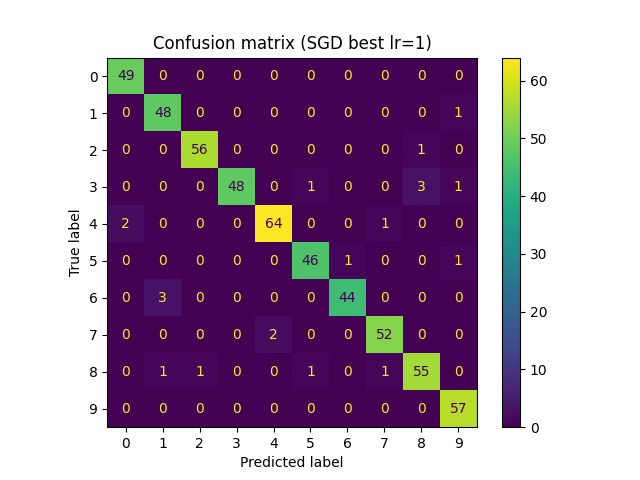
\includegraphics[width=\linewidth]{confusion-matrix-sgd-final-model.png}

            \column{0.4\paperwidth}
            \centering
            \begin{itemize}
                \item Train accuracy: $0.983$
                \item Test accuracy: $0.961$
                \item Training Time: 30ms
            \end{itemize}
        \end{columns}
    \end{frame}
       \begin{frame}
        \frametitle{Results with FGD}
        We trained a full gradient descent reference model for $300$ iterations with a learning rate of $\eta_k = 1$ on a random training set of $70\%$ of the data. The remaining $30\%$ was used as a test set.
        \begin{columns}
            \column{0.5\paperwidth}
            \centering
            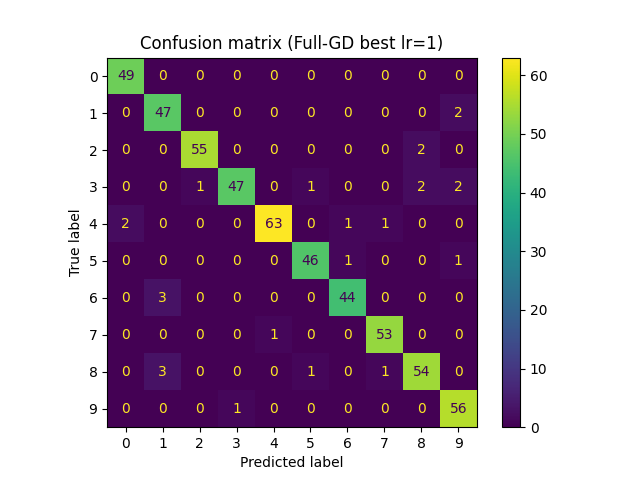
\includegraphics[width=\linewidth]{confusion-matrix-fgd-final-model.png}

            \column{0.5\paperwidth}
            \centering
            \begin{itemize}
                \item Train accuracy: $0.957$
                \item Test accuracy: $0.952$
                \item Training Time: 90ms
            \end{itemize}
        \end{columns}
    \end{frame}
    \begin{frame}
        \frametitle{Convergence Comparison}
        \begin{columns}[T]
            \column{0.5\paperwidth}
            \centering
            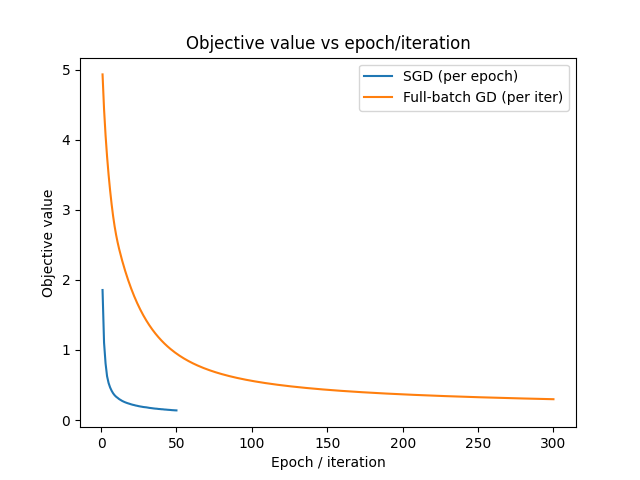
\includegraphics[width=\linewidth]{objective-value-vs-epoch.png}

            \column{0.5\paperwidth}
            \centering
            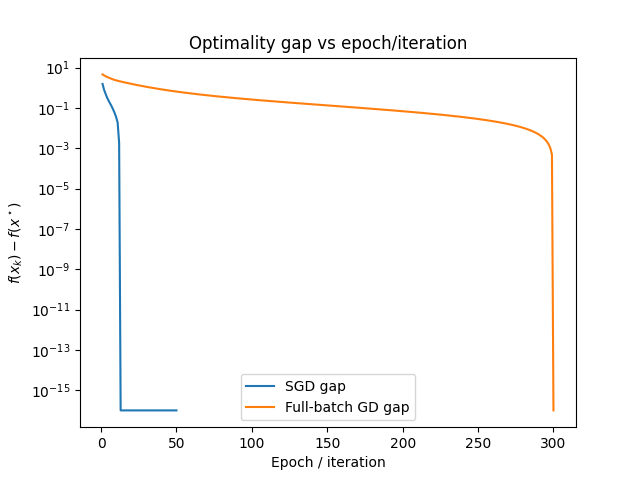
\includegraphics[width=\linewidth]{optimality-gap-vs-epoch.png}
        \end{columns}
    \end{frame}
    \begin{frame}
        \frametitle{Different batch sizes - I}
        \vspace{-0.5cm}
        \begin{figure}
            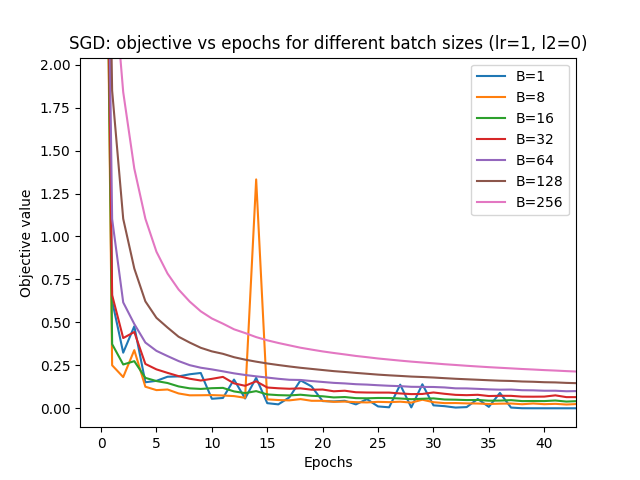
\includegraphics[scale=0.55]{sgd-batch-sizes.png}
        \end{figure}
        Result: Larger batch sizes lead to less noisy gradient estimates but also less frequent updates to the model.
    \end{frame}
    \begin{frame}
        \frametitle{Different batch sizes - II}
        \begin{columns}
            \column{0.5\paperwidth}
            \centering
            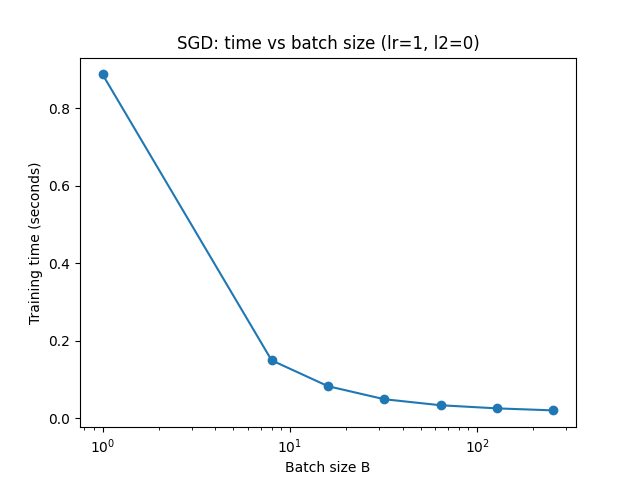
\includegraphics[width=\linewidth]{sgd-time-batch.png}

            \column{0.5\paperwidth}
            \centering
            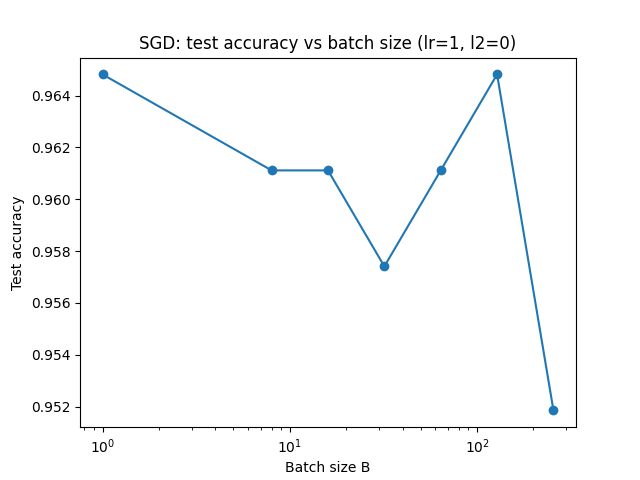
\includegraphics[width=\linewidth]{sgd-batch-accuracy.png}
        \end{columns}
    \end{frame}
    \begin{frame}
        \frametitle{Different $L^2$-regularization parameters}
        \vspace{-0.5cm}
        \begin{columns}
            \column{0.5\paperwidth}
            \centering
            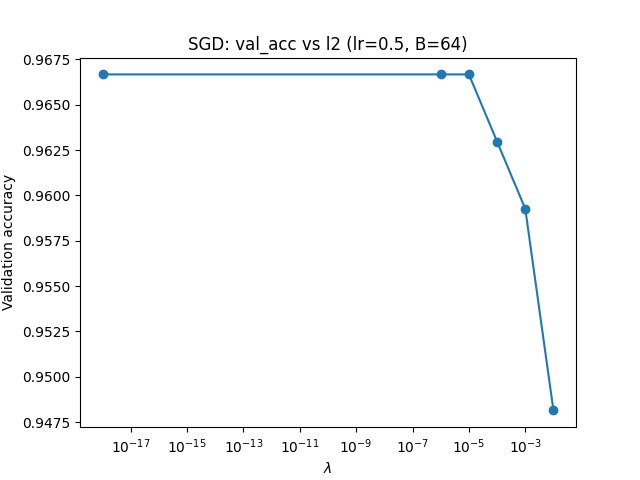
\includegraphics[width=\linewidth]{sgd-reg-accuracy.png}

            \column{0.5\paperwidth}
            \centering
            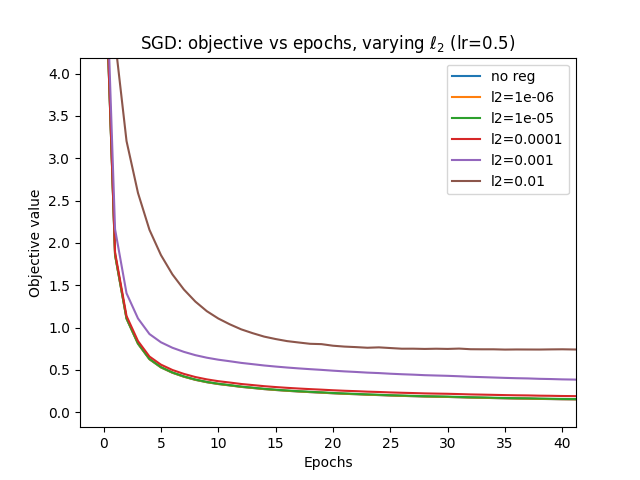
\includegraphics[width=\linewidth]{sgd-reg.png}
        \end{columns}
    \end{frame}




	

	
\end{document}